\section{Echtzeitumgebung}

Das \textit{Smart Warehouse} lehnt sich an ein großes Warenhaus an, bei dem Produkte nicht in Kartons verpackt, sondern als ganzes auf Regalen angeordnet sind, ähnlich wie bei \textit{Baumarkt} oder \textit{Selgros}. Im Rahmen des Projektes wurde sich exemplarisch auf Flaschen konzentriert, dabei wurden neun Kategorien bestimmt (siehe Abbildung \ref{categories}). 

\begin{figure}[htb]
	\subfigure[Saskia Wasser Klein]{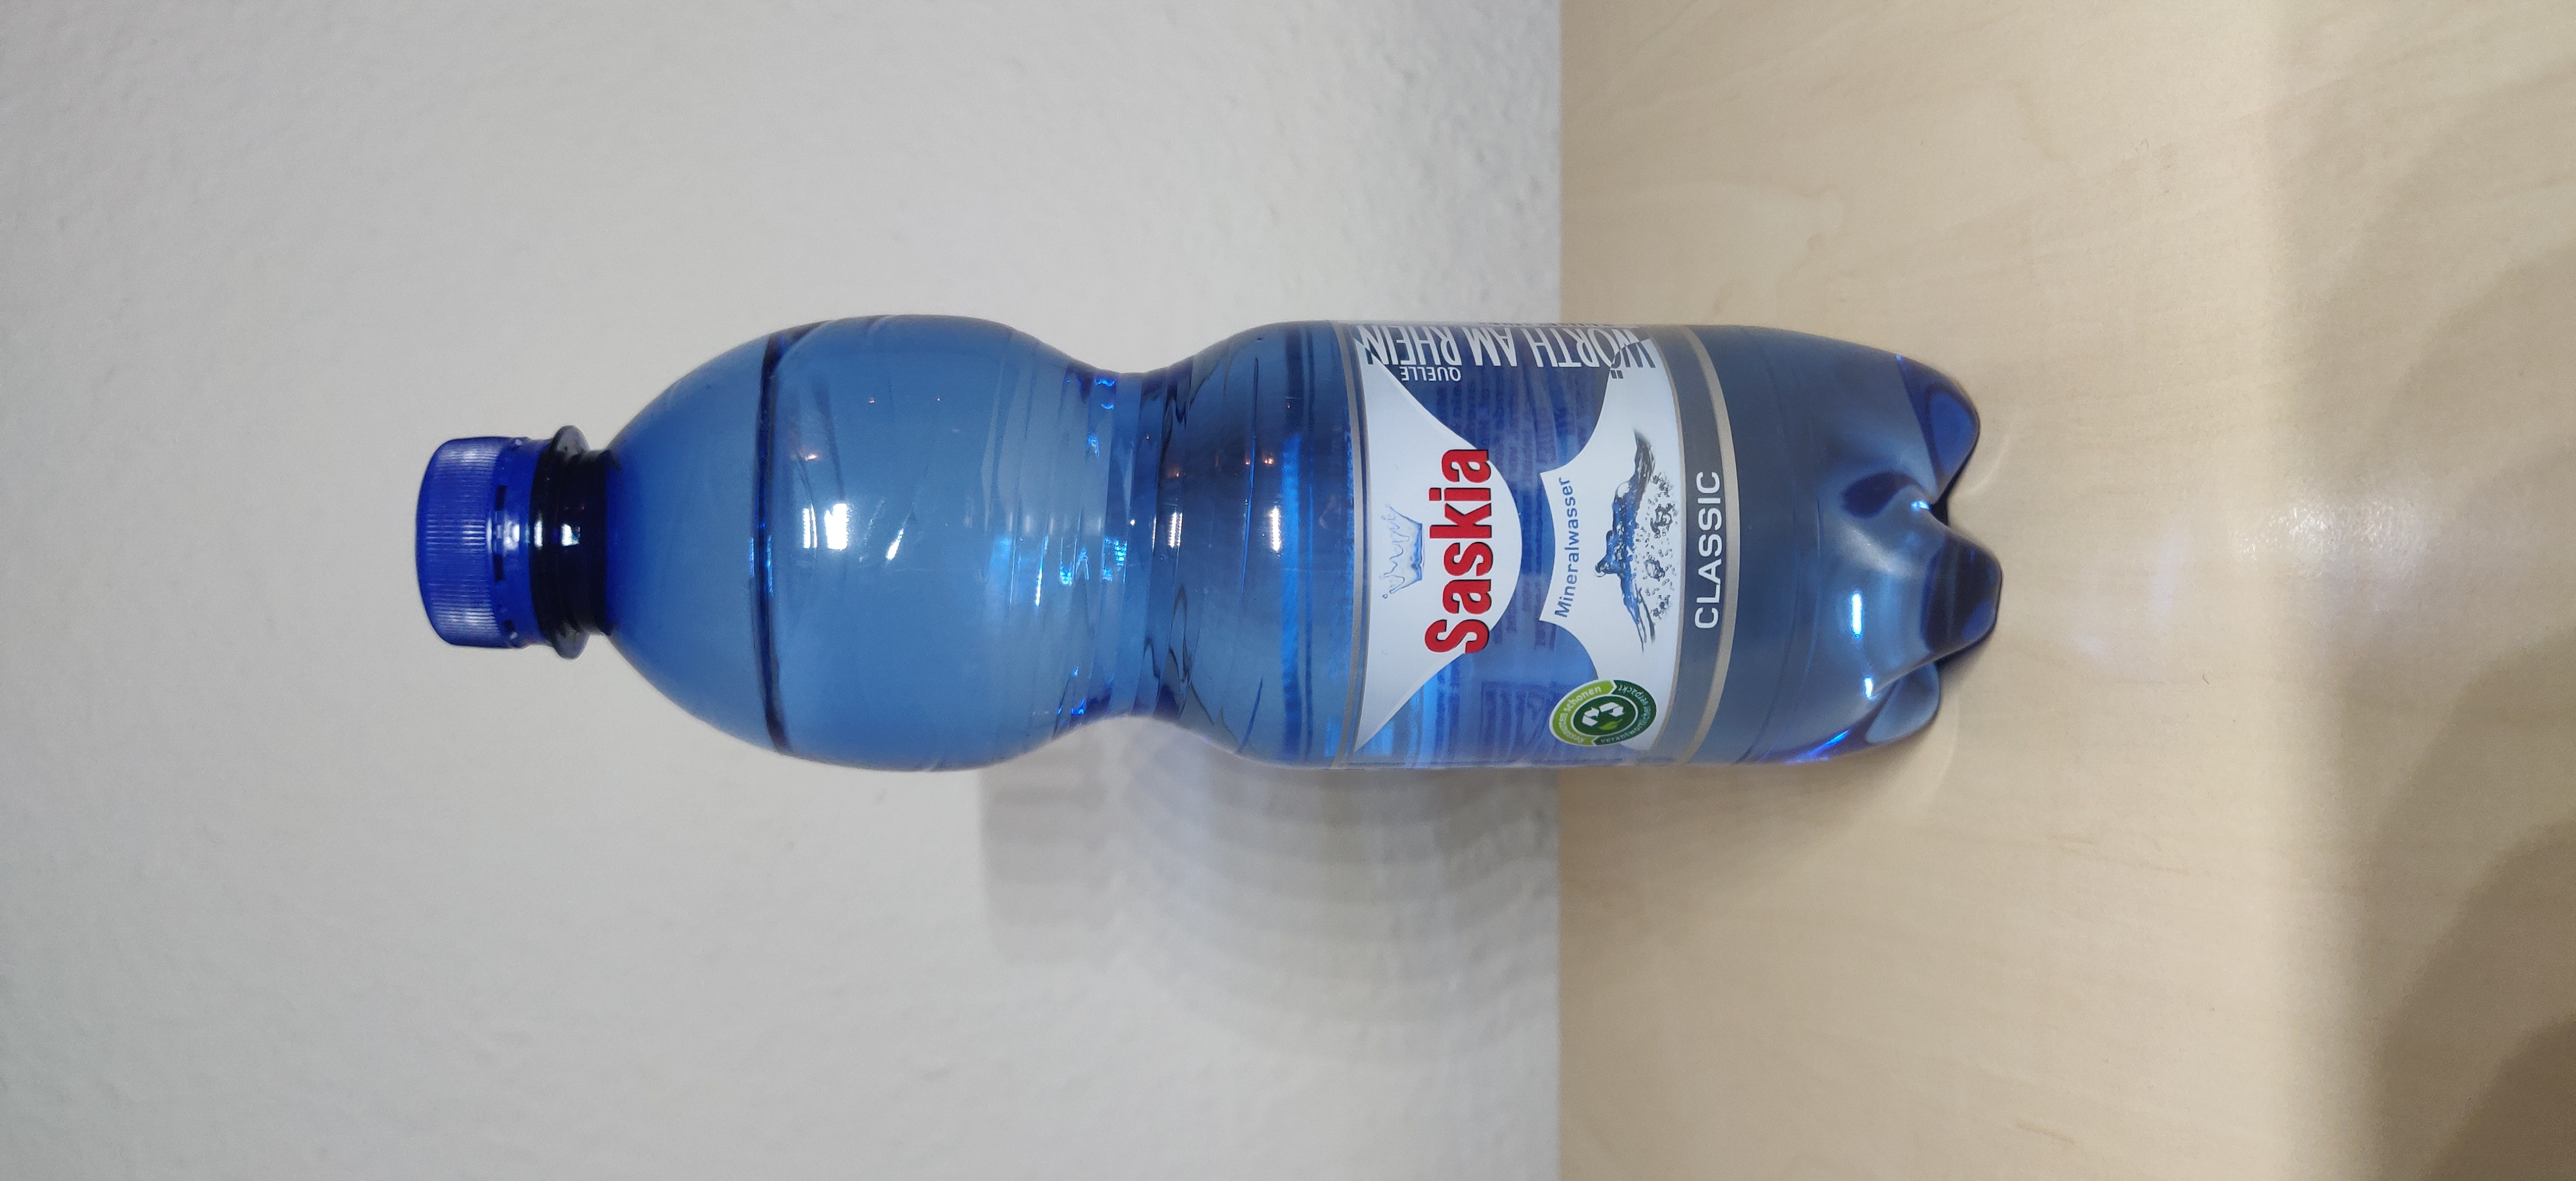
\includegraphics[width=0.32\textwidth]{Bilder/wasser_klein.jpg}}
	\subfigure[Saskia Wasser Groß]{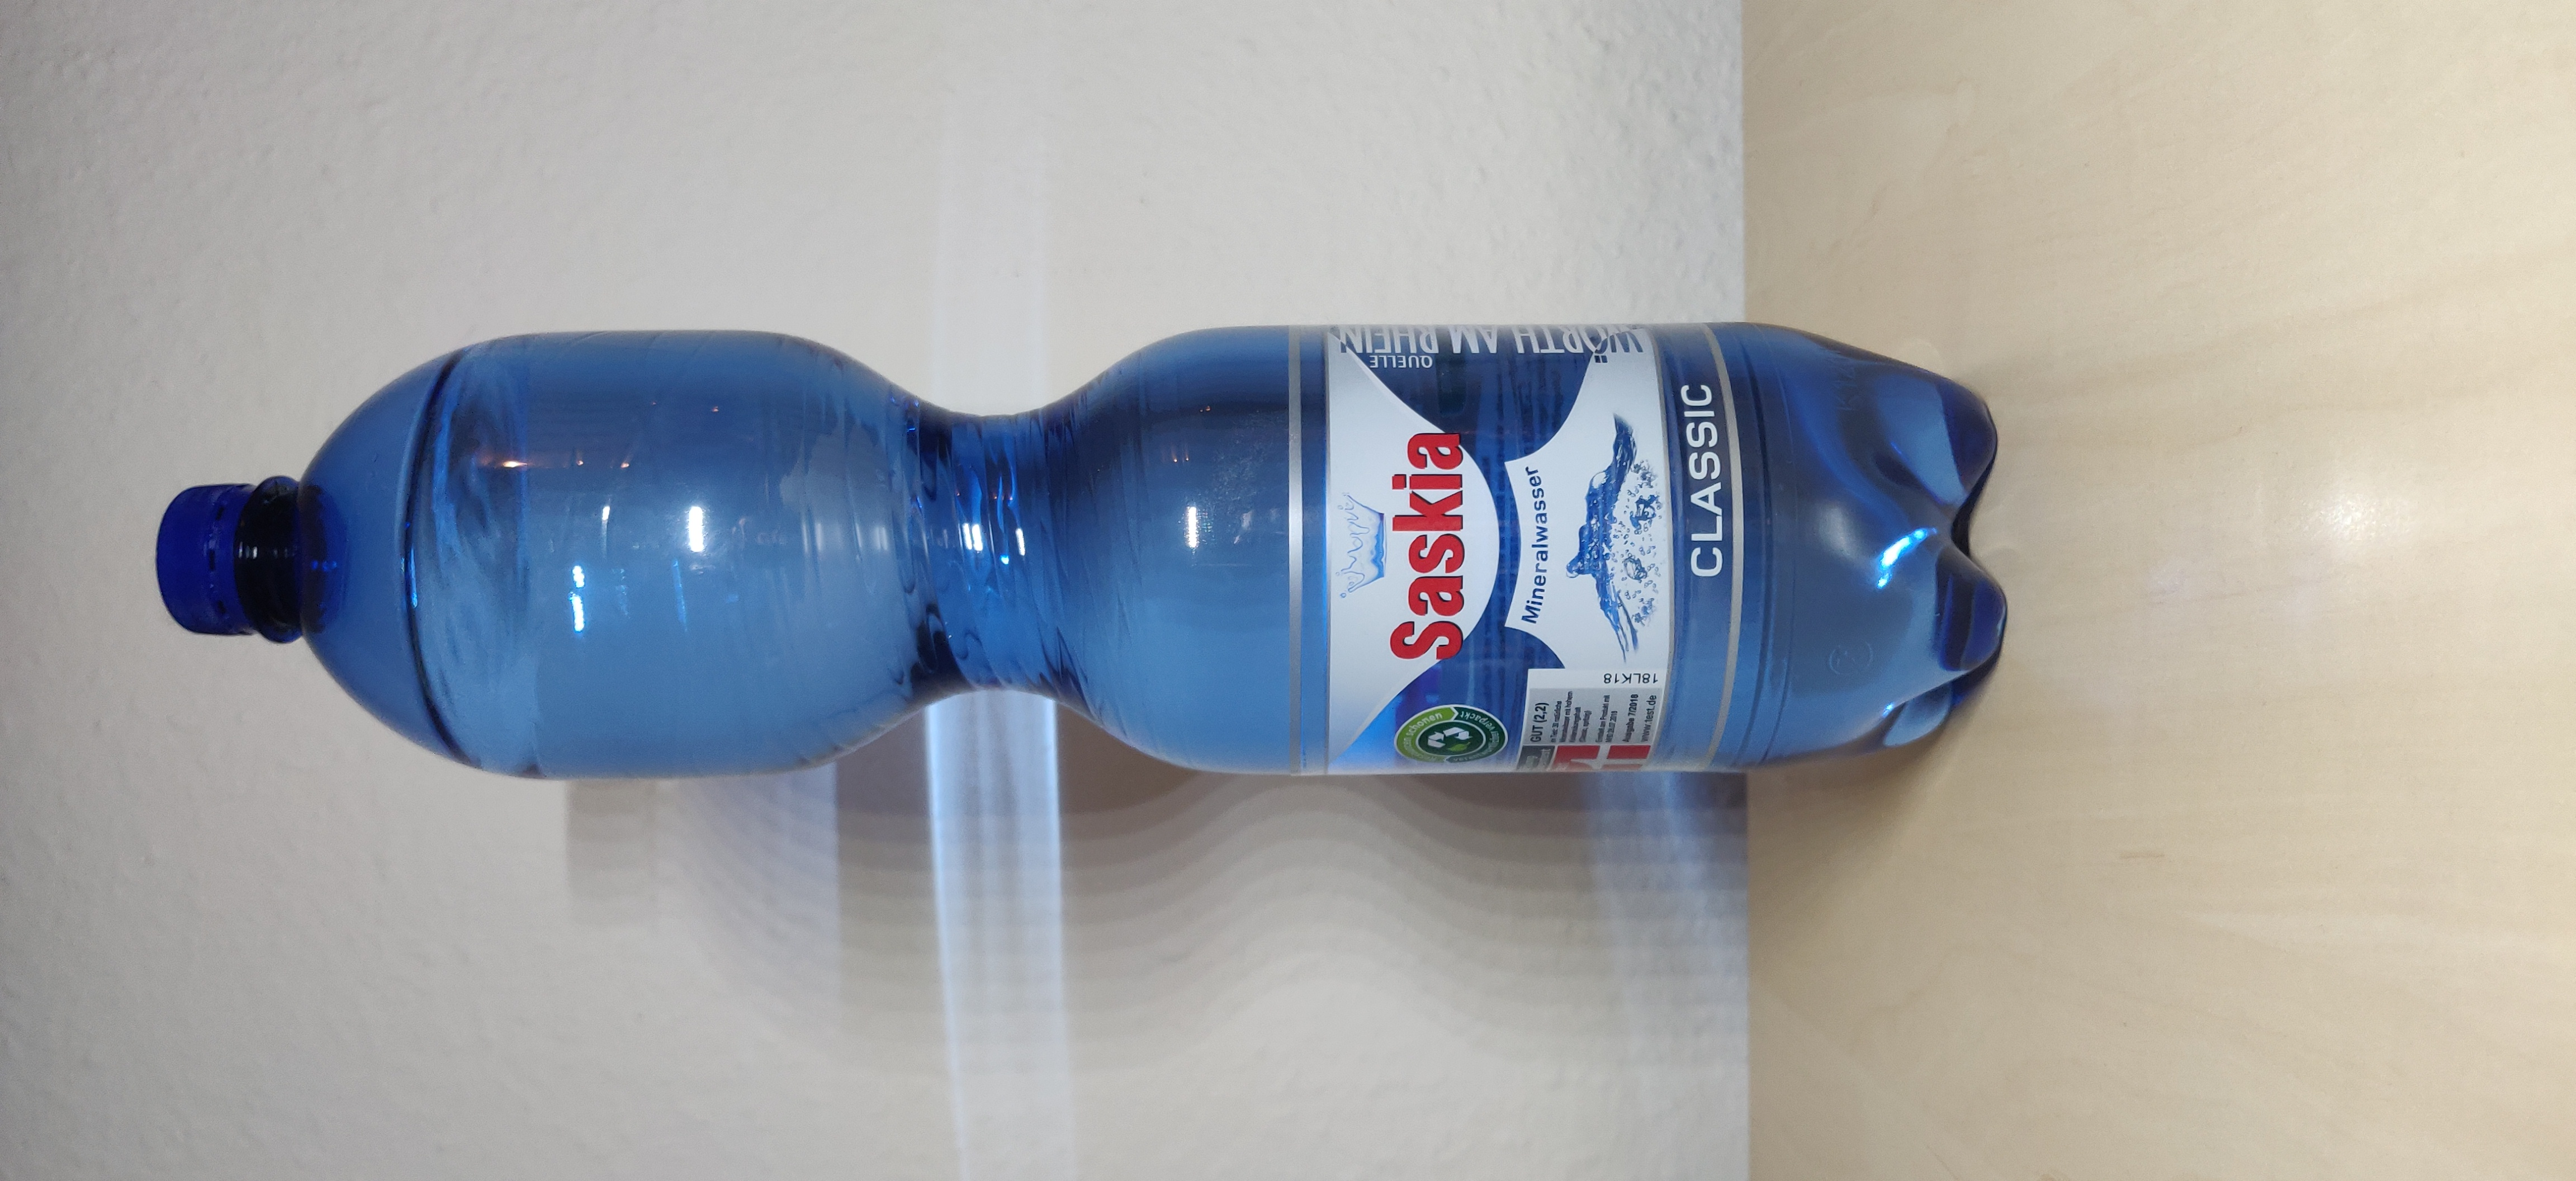
\includegraphics[width=0.32\textwidth]{Bilder/wasser_gross.jpg}}
	\subfigure[Pepsi Cola Klein]{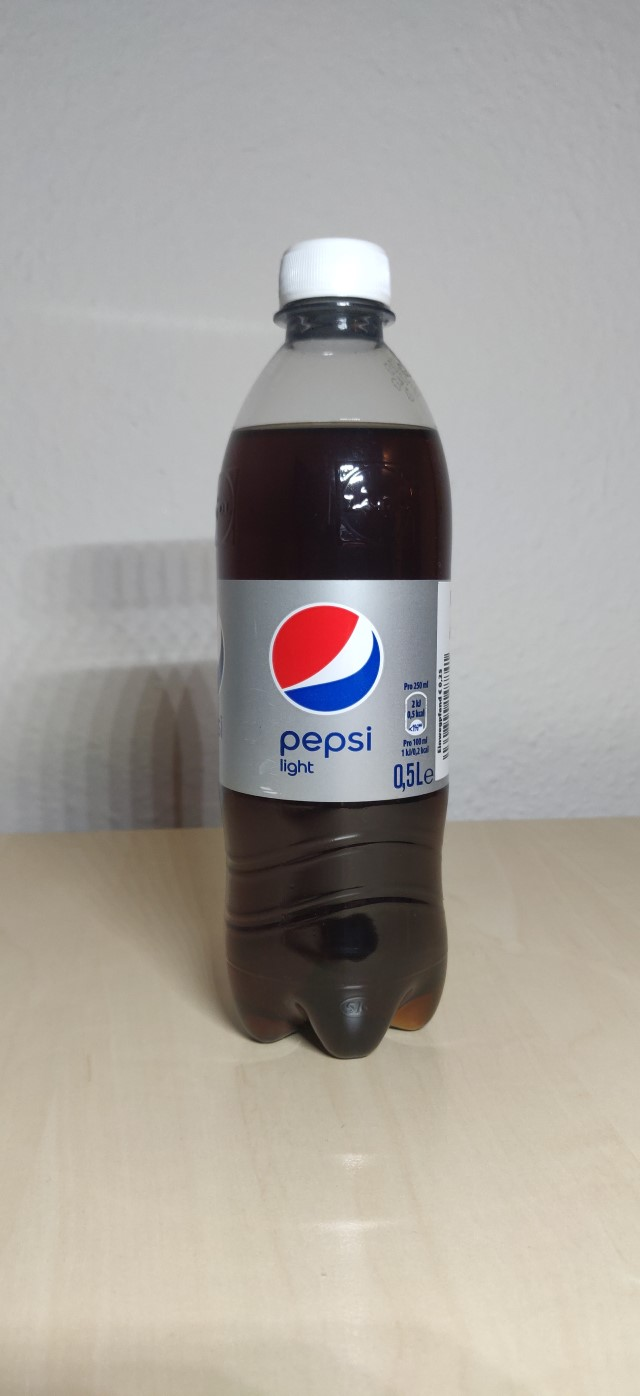
\includegraphics[width=0.32\textwidth]{Bilder/cola_klein.jpg}}
	\subfigure[Pepsi Cola Groß]{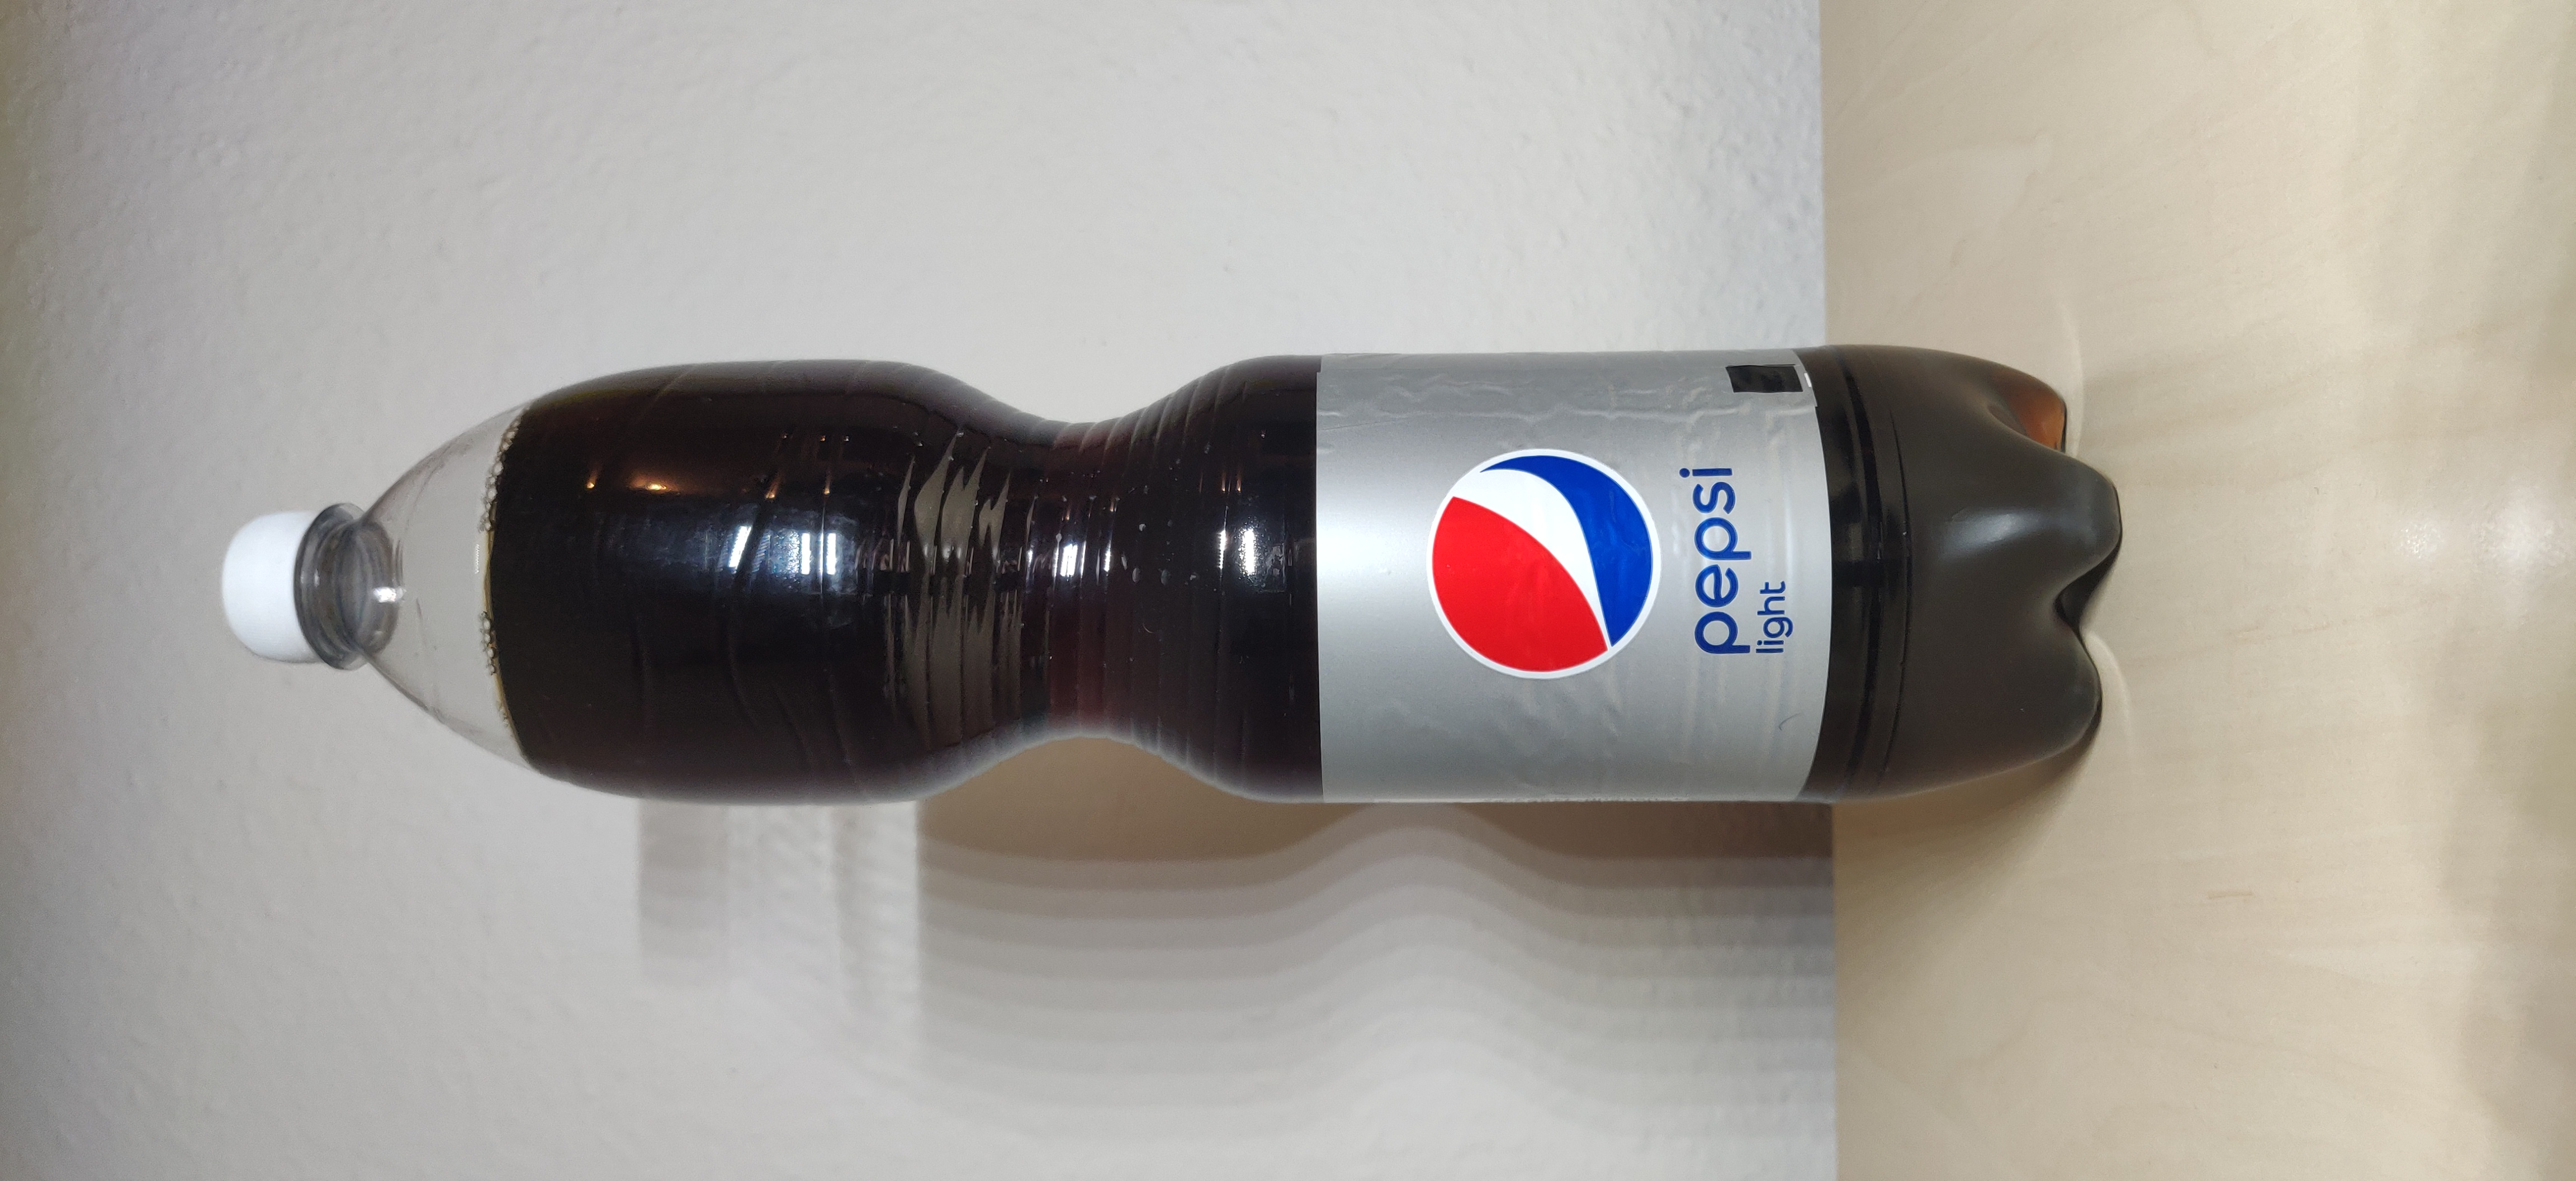
\includegraphics[width=0.32\textwidth]{Bilder/cola_gross.jpg}}
	\subfigure[ISO]{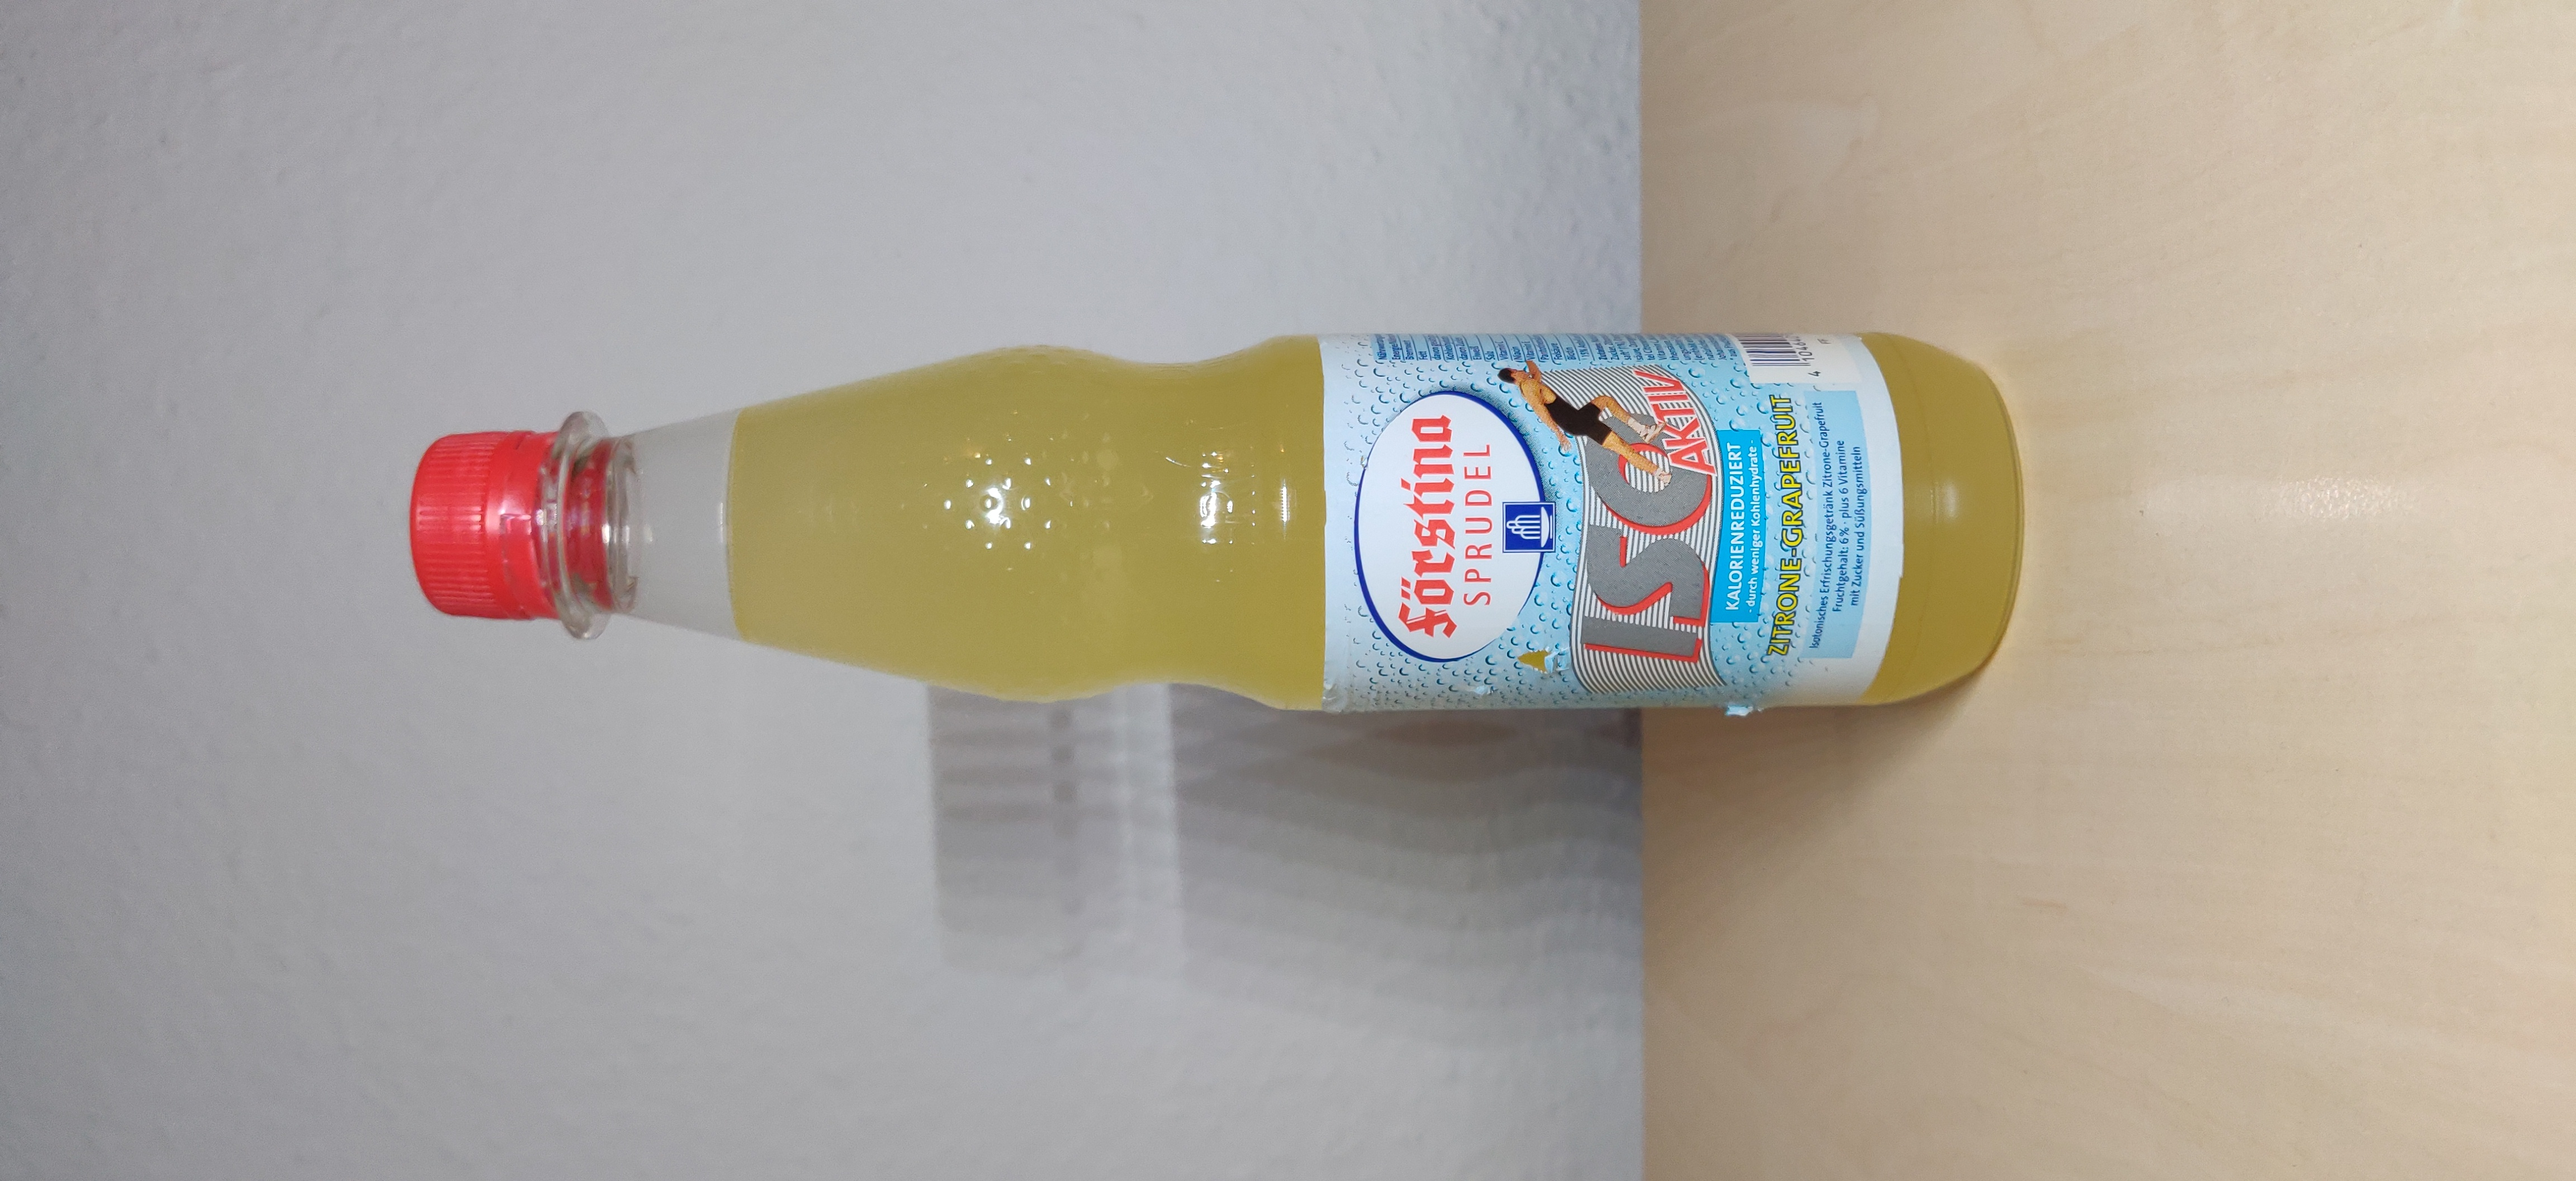
\includegraphics[width=0.32\textwidth]{Bilder/iso.jpg}}
	\subfigure[ACE]{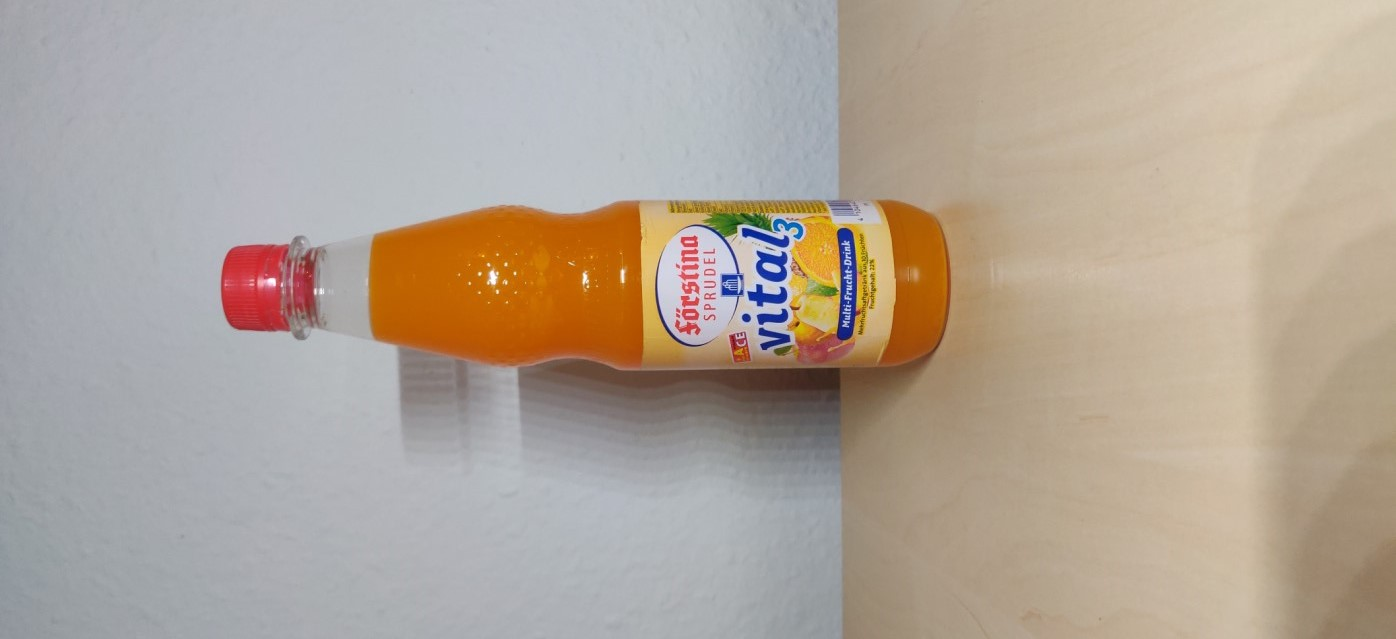
\includegraphics[width=0.32\textwidth]{Bilder/ace.jpg}}
	\subfigure[Stenger Johannisbeerschorle]{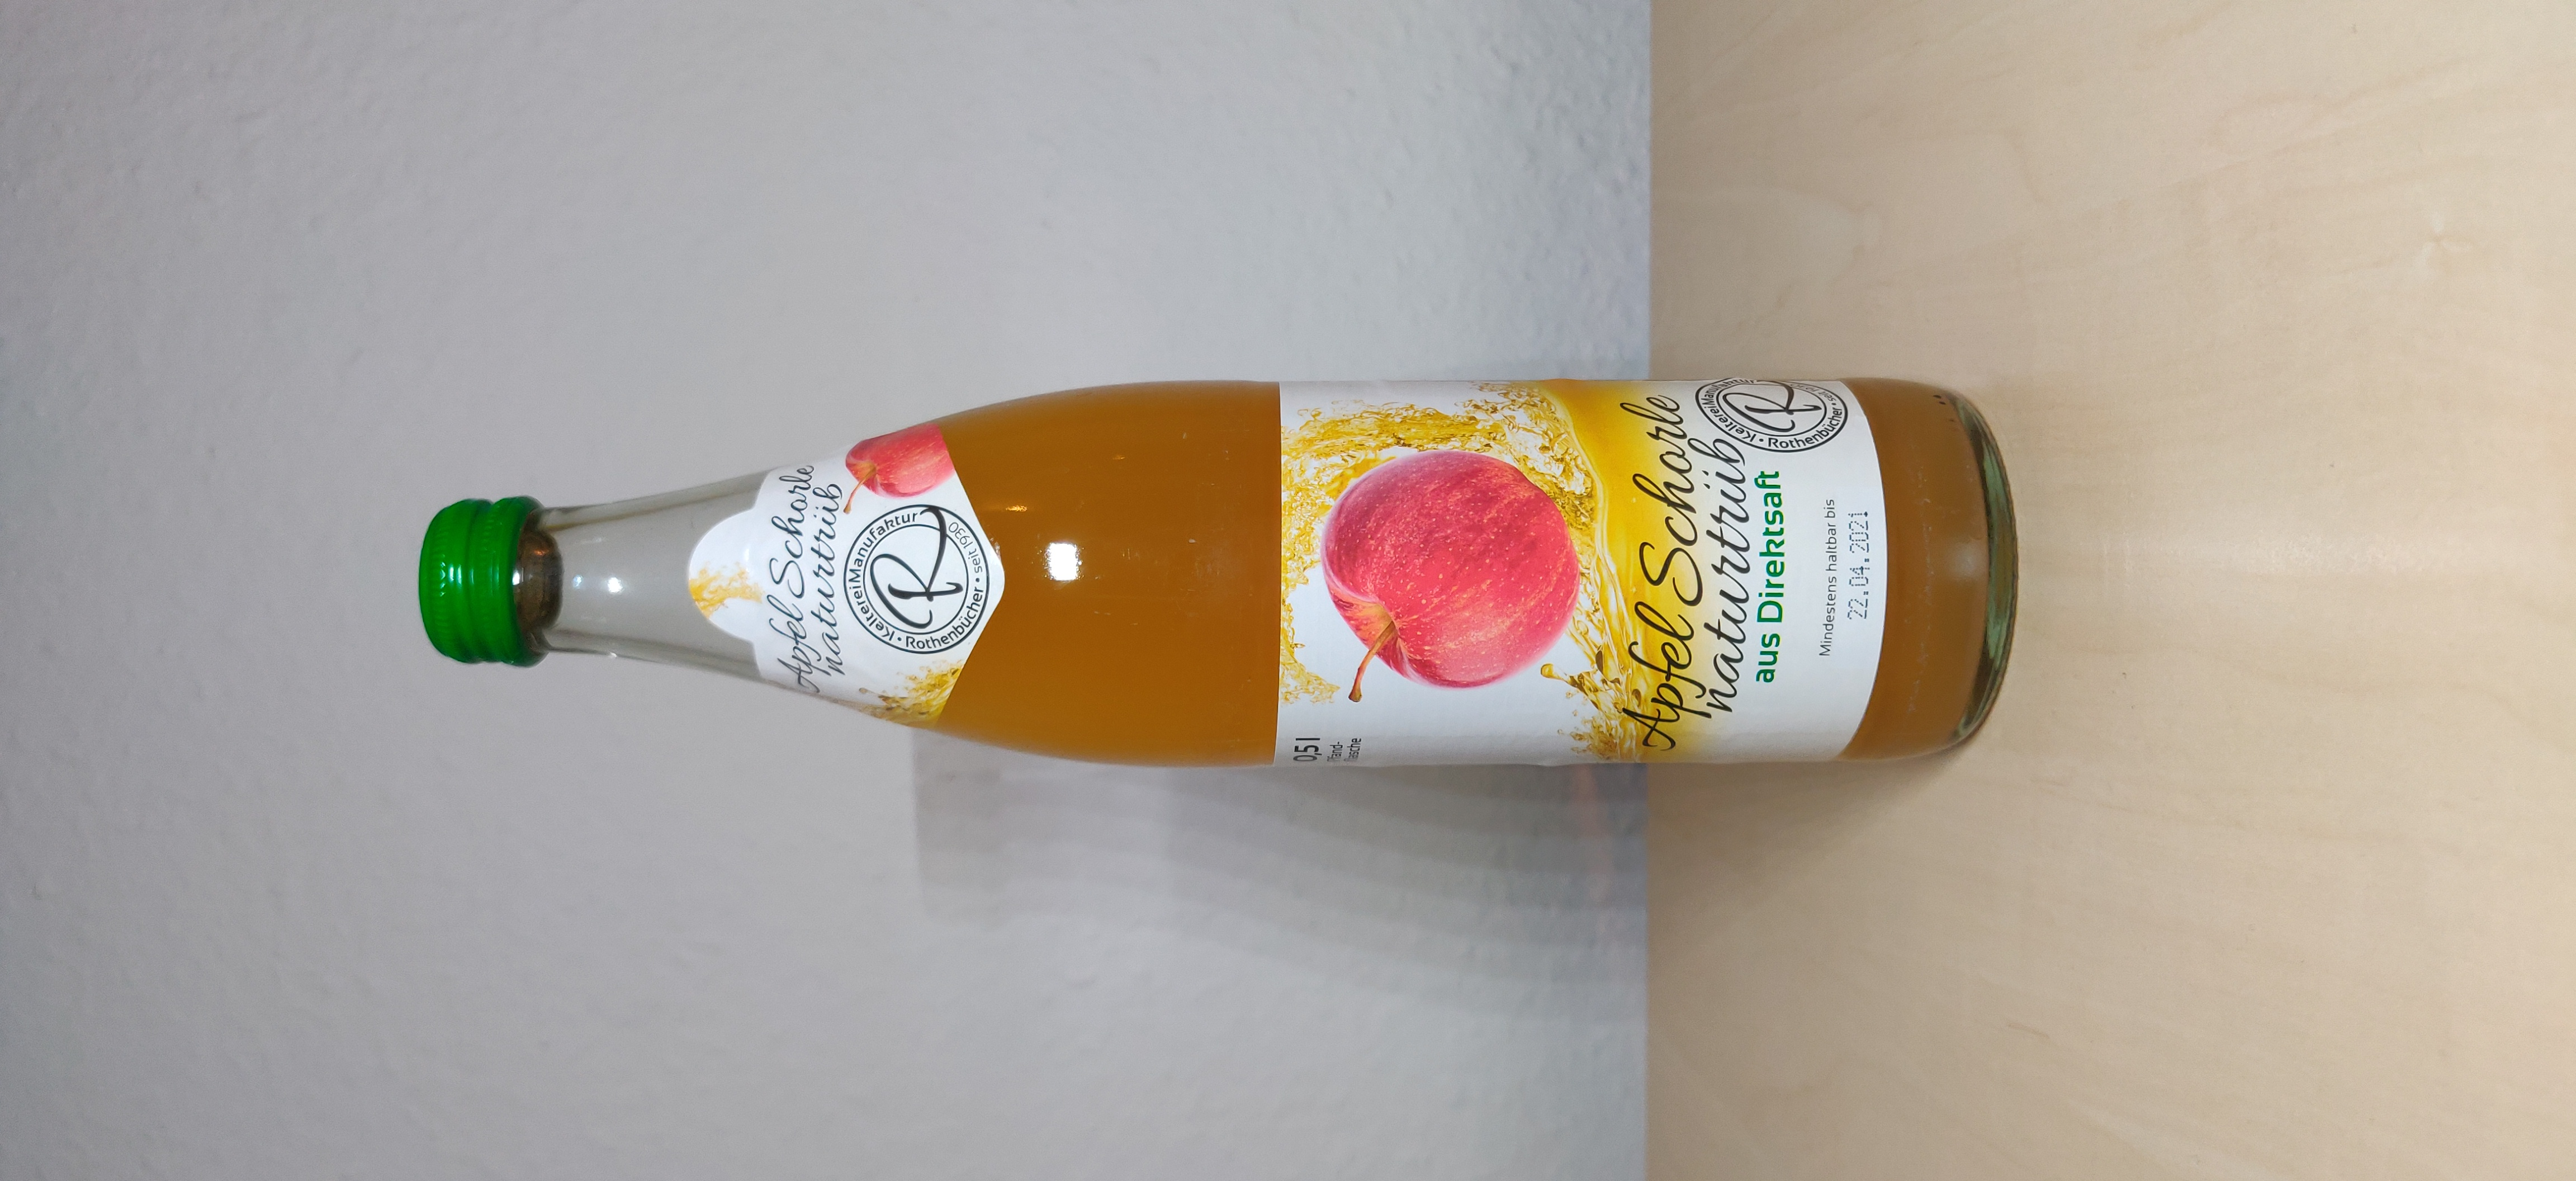
\includegraphics[width=0.32\textwidth]{Bilder/johannisbeerschorle.jpg}}
	\subfigure[Stenger Apfelsaftschorle]{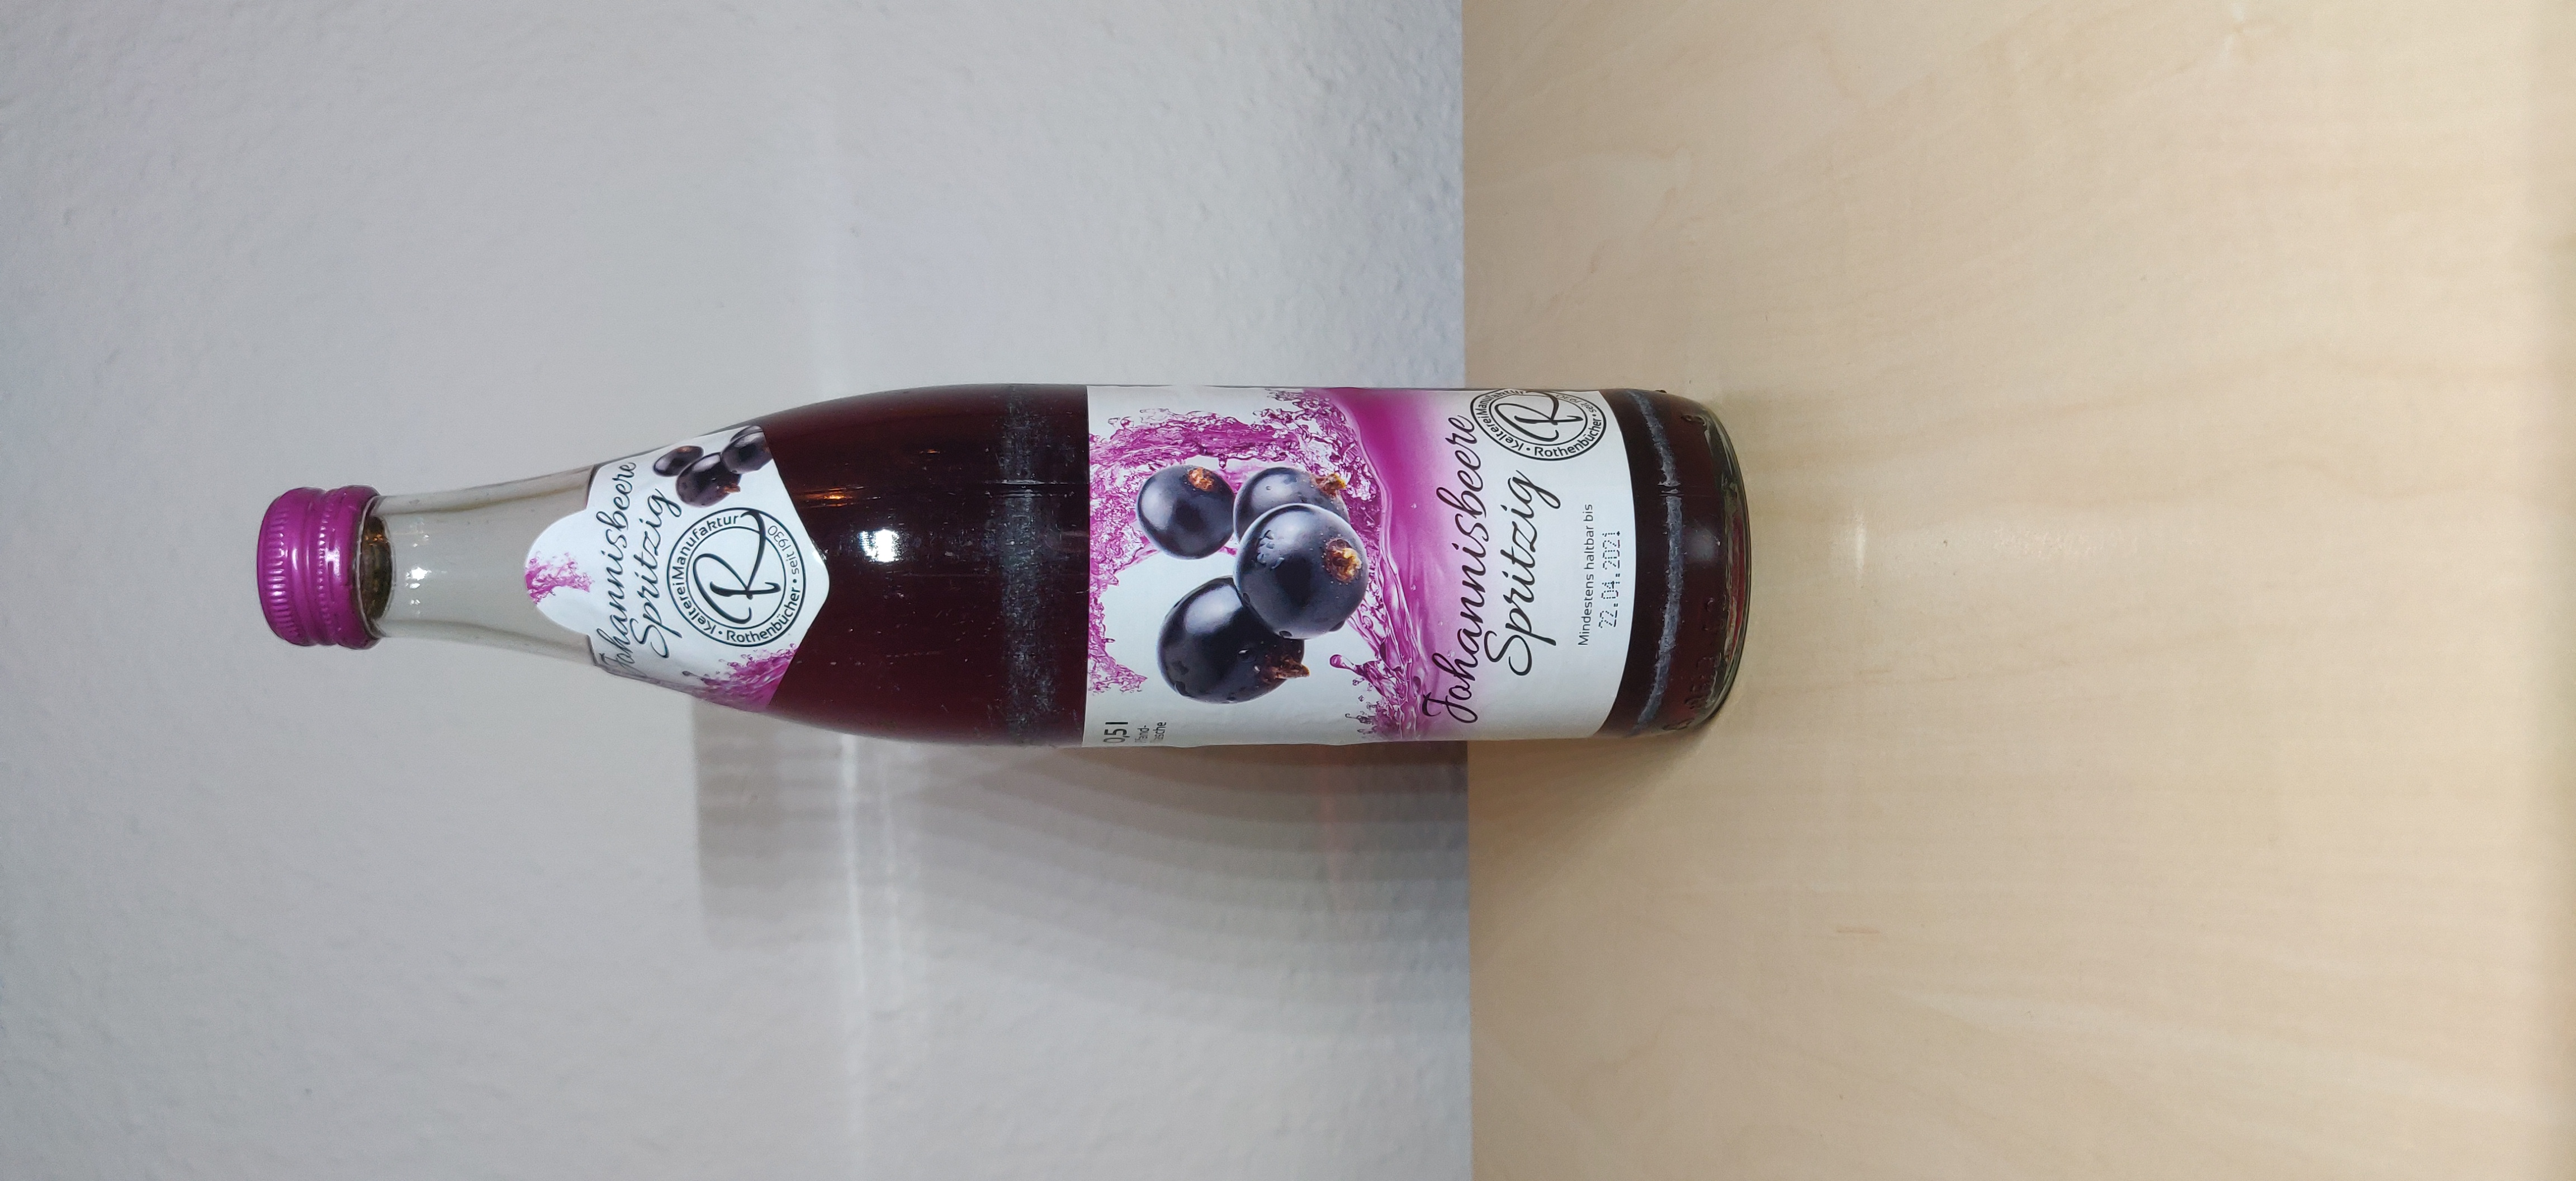
\includegraphics[width=0.32\textwidth]{Bilder/apfelsaftschorle.jpg}}
	\subfigure[Vitamalz Malzbier]{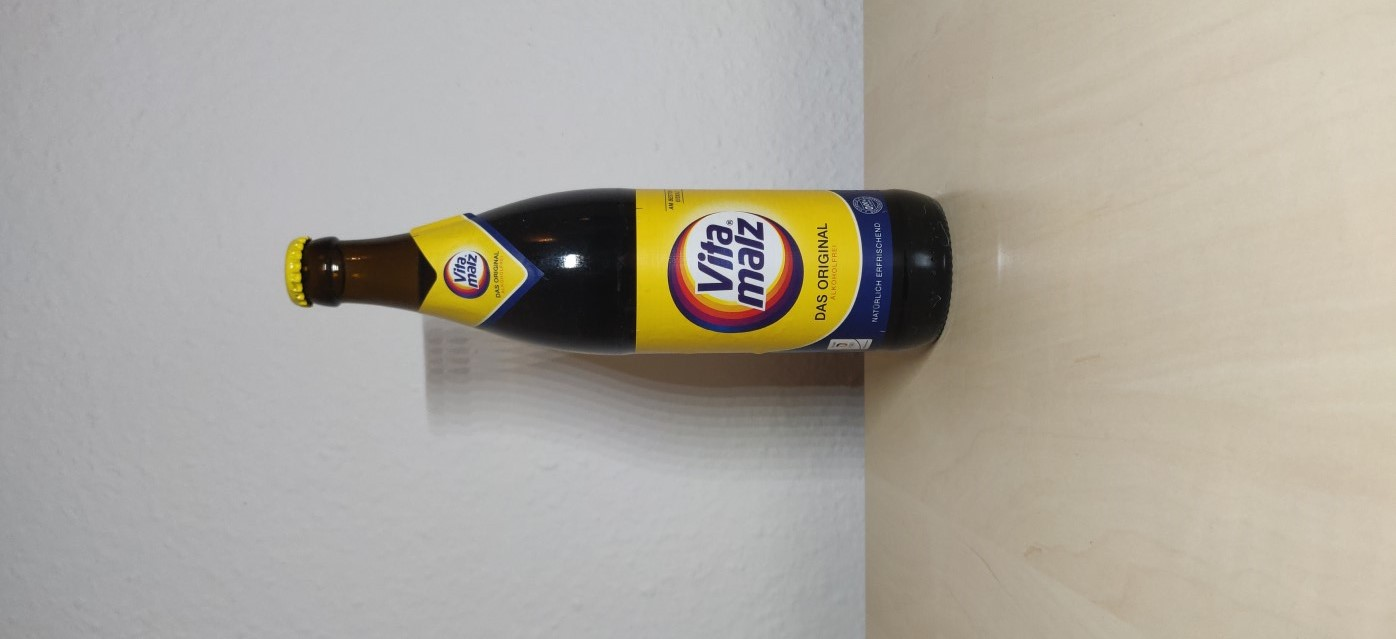
\includegraphics[width=0.32\textwidth]{Bilder/malzbier.jpg}}
	\caption{Die neun Kategorien}
	\label{categories}
\end{figure}

Der Datensatz besteht aus 1000 annotierten Bildern. Die Bilder besitzen eine Auflösung von 2112x4608 Pixels mit einer Farbtiefe von 24 Bit. Alle neuen Kategorien sind nahezu gleich häufig im Datensatz vorhanden. 

Im initialen Datensatz sind auf 75\% der Bilder die Objekte der jeweiligen Kategorien einzeln und klar erkennbar abgebildet. Hierdurch wird erhofft, dass Modell zunächst auf die Muster der jeweiligen Objekte zu trainieren. In 12,5\% der Bilder sind die Objekte der jeweiligen Kategorien ebenso einzeln, allerdings mit unterschiedlichen Hintergründen, Beleuchtungsverhältnissen, Blickwinkeln und Entfernungen abgebildet. Je nach Umgebung wurden Bilder dieses Anteils als schwer erkennbar markiert. Um das Warenhaus zu simulieren, sind in den letzten 12,5\% der Bilder die Objekte auf Regalen angeordnet, jeweils hintereinander oder in Getränkekästen (siehe Abbildung \ref{regal}). 

\begin{figure}[ht]
	\begin{center}
		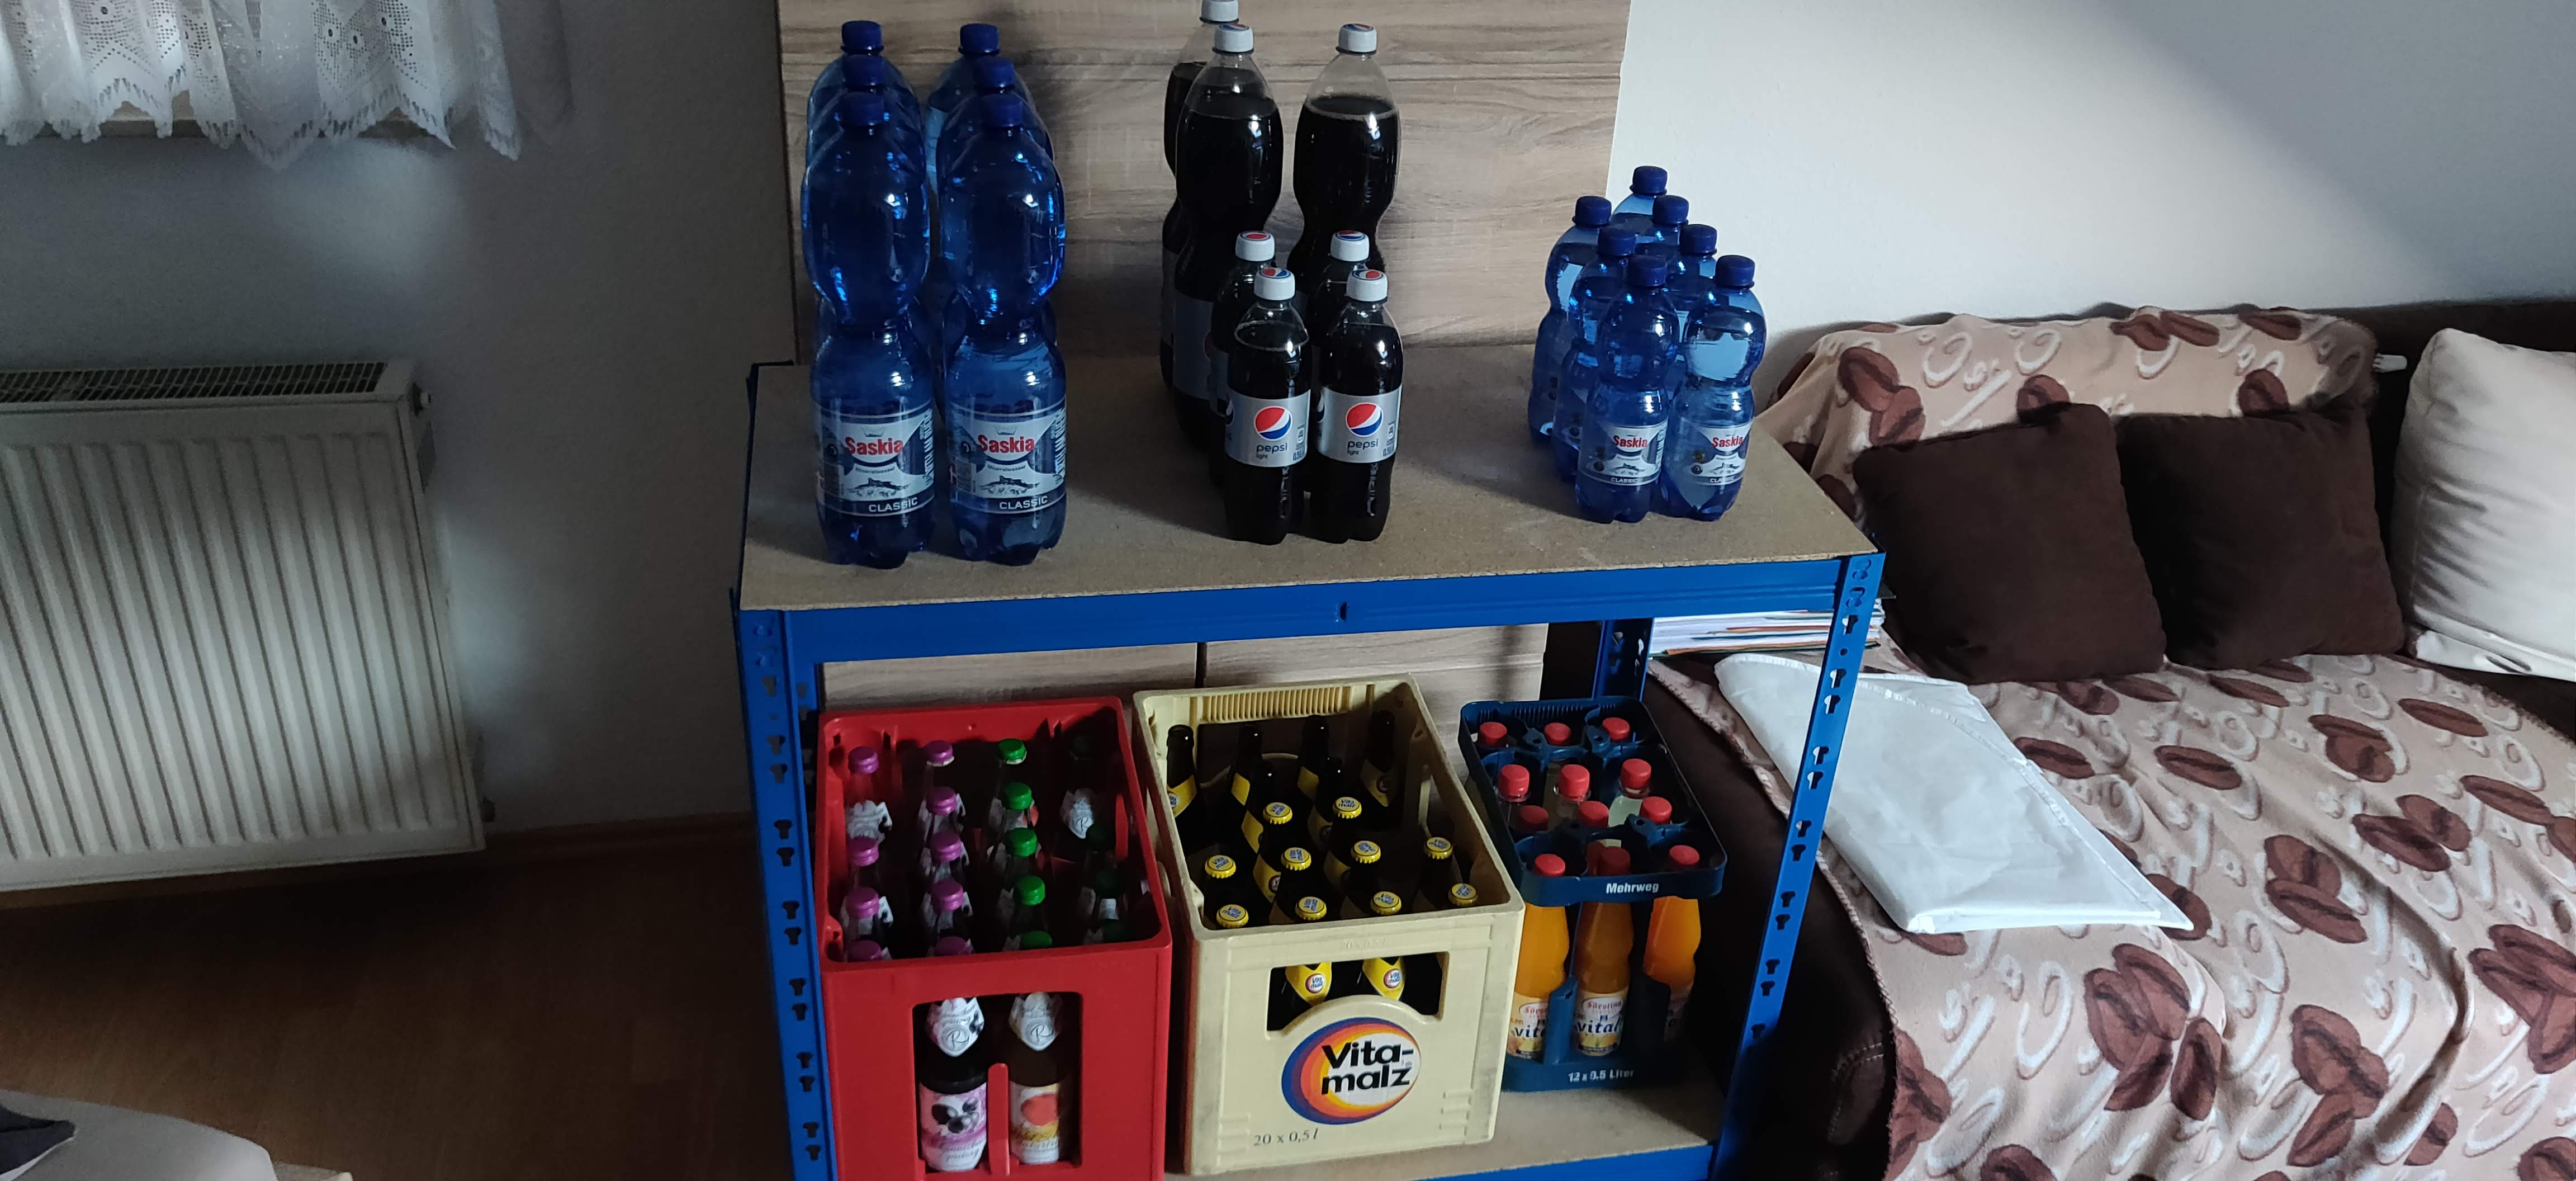
\includegraphics[width=16cm]{Bilder/regal.jpg} 
		\caption[Smart Warehouse Regal]{SmartWarehouse Regal}
		\label{regal}
	\end{center}
\end{figure}
